\documentclass[a4paper,10pt]{article}
% xelatex
%A Few Useful Packages
\usepackage{marvosym}
\usepackage{fontspec} 					%for loading fonts
\usepackage{xunicode,xltxtra,url,parskip} 	%other packages for formatting
\RequirePackage{color,graphicx}
\usepackage[usenames,dvipsnames]{xcolor}
\usepackage[big]{layaureo} 				%better formatting of the A4 page
% an alternative to Layaureo can be ** \usepackage{fullpage} **
\usepackage{supertabular} 				%for Grades
\usepackage{titlesec}					%custom \section
\usepackage{flafter}
\usepackage{multirow}
\usepackage{float}
\usepackage{ragged2e}
\usepackage[inline]{enumitem}

%Setup hyperref package, and colours for links
\usepackage{hyperref}
\definecolor{linkcolour}{rgb}{0,0.2,0.6}
\hypersetup{colorlinks,breaklinks,urlcolor=linkcolour, linkcolor=linkcolour}

%FONTS
\defaultfontfeatures{Mapping=tex-text}
%\setmainfont[SmallCapsFont = Fontin SmallCaps]{Fontin}
%%% modified for Karol Kozioł for ShareLaTeX use
\setmainfont[
Path = ../../fonts/,
BoldFont = EBGaramond-Bold.ttf,
ItalicFont = EBGaramond-Italic.ttf
]
{EBGaramond-Medium.ttf}
%%%

%CV Sections inspired by:
%http://stefano.italians.nl/archives/26
\titleformat{\section}{\Large\scshape\raggedright}{}{0em}{}[\titlerule]
\titlespacing{\section}{0pt}{3pt}{3pt}
%Tweak a bit the top margin
%\addtolength{\voffset}{-1.3cm}

%Italian hyphenation for the word: ''corporations''
\hyphenation{im-pre-se}

%-------------WATERMARK TEST [**not part of a CV**]---------------
\usepackage[absolute]{textpos}

\setlength{\TPHorizModule}{30mm}
\setlength{\TPVertModule}{\TPHorizModule}
\textblockorigin{2mm}{0.65\paperheight}
\setlength{\parindent}{0pt}

\usepackage{graphicx}

%--------------------BEGIN DOCUMENT----------------------
\begin{document}
\vspace*{-0.5cm}

\pagestyle{empty} % non-numbered pages

{\huge Alexander Hern\'andez Reyes}
\hfill
\smash{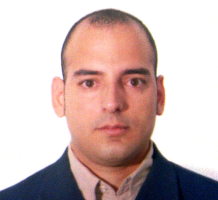
\includegraphics[width=2cm]{../../photos/Alexandercv.png}}\\
%--------------------SECTIONS-----------------------------------
%Section: Personal Data
\section{Informaci\'on personal}
\begin{tabular}{rl}
    \textsc{Tel\'efono:}     & +598 99 270 789 \\
    %\textsc{Tel\'efono:}     & +53 55 598 315 \\
    \textsc{Skype:}     & live.alxsenen \\
    \textsc{email:}     & \href{mailto:alxsenen@gmail.com}{alxsenen@gmail.com} \\
    \textsc{Linkedin:}     & \href{https://www.linkedin.com/in/alxsenen/}{https://www.linkedin.com/in/alxsenen/}
\end{tabular}

\section{Resumen}
\justify
10 a\~{n}os de experiencia, administrando sistemas y servicios, usando sistemas operativos como  \textbf{Linux} y \textbf{Windows}, \textbf{resolviendo problemas r\'apidamente}, escribiendo los pasos a seguir antes de implementar una soluci\'on. Soy \textbf{emp\'atico}, \textbf{proactivo}, de \textbf{aprendizaje r\'apido}, \textbf{serio} y \textbf{responsable}. Amplia \textbf{vocaci\'on de servicio}, dispuesto a \textbf{ayudar al equipo} y \textbf{dar lo mejor} de mi.

%Section: Work Experience at the top
\section{Experiencia laboral}
\begin{tabular}{r|p{11cm}}
\emph{02/2022 – Presente } & Ingeniero Devops, Soho Uruguay \\
	
\textsc{}&\footnotesize{Configuraci\'on y manejo de clusters \textbf{EKS}.}\\&
\footnotesize{\textbf{CI/CD} mediante pipelines usando \textbf{Azure Devops}.}\\&
\footnotesize{Despliegue y configuraci\'on de infraestructura sobre \textbf{AWS} mediante \textbf{Terraform}.}\\
	
\multicolumn{2}{c}{} \\	
\emph{12/2021 – 02/2022 } & Ingeniero Devops, Inswitch, Uruguay \\
\emph{11/2019 – 11/2021} & Administrador de sistemas - SONDA, Uruguay \\
\emph{05/2018 – 09/2019} & Administrador de sistemas - ETECSA, Cuba \\
\emph{06/2014 – 05/2018} & Administrador de sistemas - DATYS, Cuba \\
\emph{09/2013 – 09/2014} & Administrador de sistemas - UCI, Cuba \\
\emph{09/2010 – 09/2013} & T\'ecnico en seguridad inform\'atica - UCI \\
\end{tabular}

\section{Education}
\begin{tabular}{r|p{11cm}}
	\emph{2017 - 2019}  &Ingenier\'ia en Telecomunicaciones y Electrónica, ISPJAE - Incomplete \\
	\emph{2017 - 2018}  & Administraci\'on avanzada de servicios sobre Linux, DATYS - Complete \\
	\emph{08/2011}  & Administraci\'on de servidores Linux II, UCI - Complete \\
	\emph{07/2010}  & Administraci\'on de servidores Linux I, UCI - Complete \\
	\emph{2004 - 2008}  & Bachiller T\'ecnico en Electr\'onica (B.Elect.), IPTOH - Complete \\
\end{tabular}

\section{Skills}
\justify
\begin{enumerate*}
	\item VMware, AWS, GCP, Azure \hspace{0.15cm}
	\item CentOS, RedHat, openSUSE, Debian, Ubuntu, Windows Servers \hspace{0.15cm}
	\item Jenkins, Gitlab, Ansible, Bash \hspace{0.15cm}
	\item Apache, Nginx, JBoss,  Wildfly \hspace{0.15cm}
	\item Jira, Confluence, Bitbucket \hspace{0.15cm}
	\item MySQL, PostgreSQL \hspace{0.15cm}
	\item DevOps Jr. Docker, Kubernetes \hspace{0.15cm}
	\item Troubleshooting
\end{enumerate*}

\section{Idiomas}
\justify
- English - Intermedio\\
- Spanish - Nativo

\section{Proyectos}
\justify

1. \href{http://ecolehavane.org}{Sitio oficial de la Alianza Francesa en la Habana} \\
2. \href{http://www.ciarp.org/xx}{Sitio oficial del 20 Congreso de Reconocimiento de Patrones (CIARP 2015))}\\
3. \href{http://www.ciarp.org/xxi}{Sitio oficial del 21 Congreso de Reconocimiento de Patrones (CIARP 2016)} \\
4. \href{http://acrp.cenatav.co.cu}{Asociaci\'on Cubana de Reconocimiento de Patrones (ACRP)} \\

\end{document}
